\documentclass[runningheads,a4paper]{llncs}

\usepackage{amssymb}
\setcounter{tocdepth}{3}
\usepackage{graphicx}
\usepackage{url}
\usepackage[spanish]{babel}



% ! META INFO
% ? Title of the doc
\title{ReTex: implementación de un sistema de recuperación de información basada en texto.}
\titlerunning{ReTex}
% ? authors of the doc
\author{Frank Abel Blanco Gómez - C312\\Ariel Alfonso Triana Pérez - C311}
\authorrunning{F. Blanco, A. Triana}
% ? institute of authors
\institute{Facultad de Matemática y Computación (MATCOM),\\
Universidad de La Habana\\
San Lázaro y L. Vedado. La Habana. Cuba\\
\url{frank.blanco@estudiantes.matcom.uh.cu}\\
\url{ariel.triana@estudiantes.matcom.uh.cu}}

\begin{document}
    \mainmatter 
    \maketitle

    \begin{abstract}
        La Recuperación de Información en Texto es una rama de la investigación multidisciplinaria donde se pretende como primer objetivo  extraer información representada en documentos digitales de texto. En el presente se propone un modelo de recuperación de información basado en el modelo vectorial que cuenta con una interfaz gráfica. El modelo propuesto es rápido y recupera una fracción buena de documentos relevantes aplicando técnicas de lemantización y eliminación de stopwords en los documentos. El ranking construido como respuesta a las consultas del usuario se hace utilizando las técnicas de Top-rank y Threshold-rank. Además se evalua el sistema de forma crítica proponiendo mejoras al sistema.
        \keywords{Recuperación de Información en texto, Modelo vectorial, Tf-Idf}
    \end{abstract}

    % ? Include sections using the following convention:
    % ?  - Add a file *.tex in sections folder
    % ?  - Include file in main like \input
    \section{Introducción}

La Búsqueda y Recuperación de Información (ISR, por sus siglas en inglés: Information Search and Retrieval) es la rama de la ciencia encargada de buscar información en colecciones de documentos digitales. La misma explora los metadatos y el contenido de los documentos para extraer datos que permitan caracterizar la información contenida en los mismos. La ISR no solo se limita a trabajar con documentos de texto, también tiene enfoques de recuperación de información en imágenes, videos, música. \cite{mri} 

La Recuperación de Información es una rama interdisciplinaria donde generalmente trabajan un grupo de diversos científicos de la bibliotecología, arquitectura de la información, ciencia de la computación, lingüística, inteligencia artifical, archivística, entre otros.

Con la escalada de los grandes volúmenes de datos, surge la necesidad de tener sistemas que recuperen la información deseada por los usuarios, y lo hagan de forma rápida y precisa. De ahí que se dediquen grandes esfuerzos al desarrollo de sistemas que satisfagan estas necesidad.

El proceso de recuperación comienza cuando un usuario hace una consulta de información al sistema. Se entiende por consulta una afirmación formal de la información que necesita el usuario, por ejemplo: ``¿Qué leyes de similitud se deben obedecer al construir modelos aeroelásticos de aeronaves de alta velocidad calentadas?''. Una consulta de forma general no identifica un único documento dentro de la colección de los mismos, si no que identifica un conjunto de esto, donde cada uno de ellos responde a la consulta con un nivel $r$ de relevancia. 

A menudo los sistemas de recuperación desarrollan un ranking según el nivel $r$ de relevancia para una consulta y devuelven al usuario los documentos que contengan mayor $r$.
    \section{ReTex}

Retex es una propuesta de implementación de un sistema de recuperación de información textual. Retex está dividido en dos aplicaciones: 

\begin{enumerate}
    \item \textbf{Motor de búsqueda} implementado en Python utilizando una API (abreviatura de Application Programming Interface). Todo el procesamiento del motor de búsqueda se implementó en un módulo de Python cuyo nombre es \verb|retex|, y la API se implementó utilizando la librería de Python \verb|FastAPI|.
    \item \textbf{Interfaz visual} implementado en VueJS, framework para el desarrollo de frontend en aplicaciones webs.
\end{enumerate}

\subsection{Motor de búsqueda}

El motor de búsqueda se basa en el modelo vectorial de recuperación de información, el cual se define como sigue. Un Modelo Vectorial de Recuperación de Información \cite{manning} no es más que una tupla $<D, Q, F, R>$ donde:

\begin{enumerate}
    \item[$\bullet$] $D$: Vectores de los pesos asociados a los términos  de los documentos. Estos pesos $w$ son no binarios y mayores que cero ($w > 0$)
    \item[$\bullet$] $Q$: Vector de los pesos asociados a los términos de la consulta.
    \item[$\bullet$] $F$: Espacio $n$ dimensional y operaciones entre vectores del álgebra lineal
    \item[$\bullet$] $R$: Función de ranking, generalmente es el coseno entre el vector de pesos de la consulta y los vectores de los documentos.
\end{enumerate}

El motor de búsqueda implementado sigue el flujo mostrado en la Fig \ref{esq}, donde el usuario realiza una consulta $q$ en forma de texto a través de la interfaz visual. La consulta $q$ se convierte en una instancia de la clase \verb|Query|, donde se almacenan las palabras claves de la misma, y se almacenan los pesos de cada término. Esta consulta se introduce en el modelo vectorial y se calcula el ranking $R$ de los documentos relevantes a $q$, donde el documento $R_1$  es el más relevante y por lo tanto tiene mayor similitud con la consulta $q$ del usuario.

\begin{figure}\label{esq}
    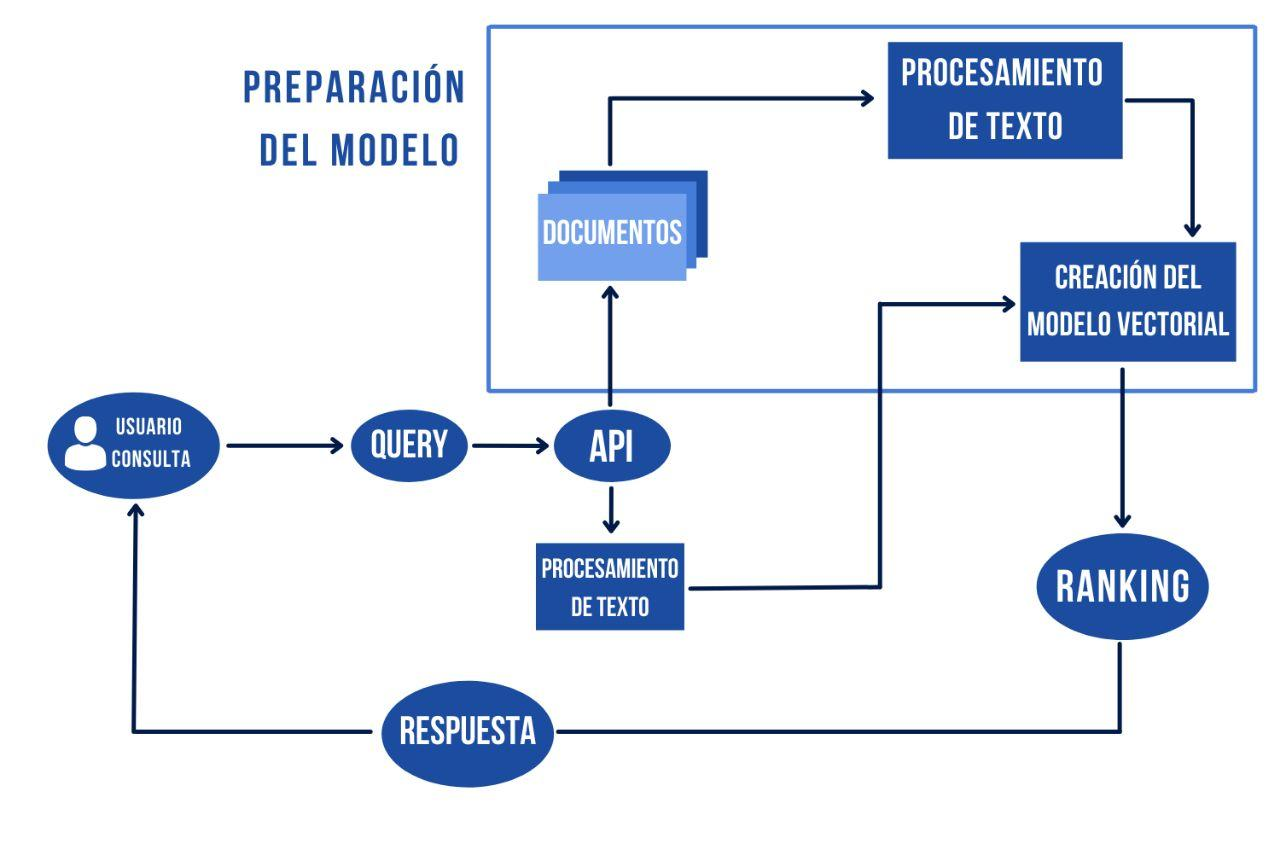
\includegraphics[width=10cm]{sections/img/esq.jpg}

    \caption{Flujo del motor de búsqueda}
\end{figure}

La preparación del modelo consiste en lo siguiente: se trabajó con la colección de documentos Cranfield \cite{cran} que cuenta con 1400 documentos y 255 consultas con la relación de relevancia de los documentos. Por tanto, se cargan todos los documentos del archivo \verb|cran.all.1400|, para ello se implementa un clase denominada \verb|CranParser| que utilizando la librería de expresiones regulares de Python \verb|re| separa todos los docuementos y sus metadatos en instancias de la clase \verb|CranDocument|. La clase anteriormente mencionada representa un documento de la colección Cranfield y su implementación es la siguiente:

\begin{verbatim}
class CranDocument(BaseDocument):
    __type__ = "cran"

    def __init__(self, id, title, text, author, editorial):
        BaseDocument.__init__(self, id, title.lower(), text.lower())
        self.author = author.lower()
        self.editorial = editorial.lower()
\end{verbatim}

Luego de tener una lista con todos los documentos de la colección se procede a procesar los textos de los documentos y posteriormente extraer las palabras claves o los términos de los documentos. 

En el procesamiento de texto se utilizó la librería de Python \verb|nltk| y se realizaron los siguientes procedimientos:

\begin{enumerate}
    \item Eliminación de los signos de puntuación.
    \item Eliminación de stopwords: palabras que no aportan información alguna al modelo, ni permiten decidir en qué categoría se debe clasificar el texto. Por ejemplo: preposiciones, conjunciones, entre otras.
    \item Normalización de los documentos a minúscula. 
    \item Aplicación de la lemantización.  La lemantización es un proceso lingüístico que consisten en dada una forma flexionada hallar el lema correspondiente. Por ejemplo: el lema de la palabra jóvenes es joven. Es decir, el lema de una palabra es aquella que se encuentra como entrada de un diccionario tradicional, esto es singular para los sustantivos, masculino singular para adjetivos, y el infinitivo para los verbos.
\end{enumerate}

Para la extracción de palabras claves se implementó una clase \verb|Indexer| que dado una colección de docuementos devuelve para cada uno los términos y sus pesos asociados. Se exploraron dos enfoques principales en la selección de palabras claves o términos:

\begin{enumerate}
    \item[$\bullet$] \verb|NaiveIndexer|, en el cual todas las palabras del documento son palabras claves.
    \item[$\bullet$] \verb|NounIndexer|, en el cual solo los sustantivos presentes en los documentos son palabras claves. En el artículo Relevance Weighting of Search Term \cite{re} se plantea que los sustantivos de un documento tienden a expresar la temática del mismo. 
\end{enumerate}

Luego de experimentar con ambos enfoques se decidió adoptar el \verb|NounIndexer| como mecanismo de selección de palabras claves para el motor de búsqueda. Posterior a todo este procesamiento se tiene un lista de vectores $K$ de palabras claves.

\begin{verbatim}
class Indexer(ABC):
  def __call__(self, docs_text: List[str]):
      vocabulary = self.extract_vocabulary(docs_text)
      vectorize = TfidfVectorizer(vocabulary=vocabulary)
      weight = vectorize.fit_transform(docs_text)
      idf = vectorize.idf_
      tf = [w / idf for w in weight]
      return (weight, idf, tf, vectorize.get_feature_names_out())
  @abstractmethod
  def extract_vocabulary(self, docs_text: List[str]) -> List[str]:
    pass

class NounIndexer(Indexer):
  def extract_vocabulary(self, docs_text: List[str]) -> List[str]:
    is_noun = lambda pos: pos[:2] == 'NN'
    stop_words = set(stopwords.words('english'))
    nouns: Set[str] = set()
    for doc in docs_text:
        tokenized = word_tokenize(doc)
        tokenized = [WordNetLemmatizer().lemmatize(w) for w in tokenized]
        tokenized = [token for token in tokenized if not token in stop_words]
        for (word, pos) in pos_tag(tokenized):
            if is_noun(pos):
                nouns.add(word)
    return list(nouns)
\end{verbatim}

\subsubsection{Ponderación de términos en el motor de búsqueda}

Luego de tener los términos de cada documento es necesario obtener los pesos asociados a cada uno de estos términos. Para ello se utilizó la clase \verb|TfIdfVectorizer| \cite{tf} \cite{tfidf} de la librería \verb|sklearn| de Python, que tiene el siguiente funcionamiento implementado de forma eficiente:

Se calcula la frecuencia $f_i$ de aparición de cada término en los documentos y se calcula el $tf_{ij}$ que corresponde a la frecuencia normalizada del término $i$ en el docuemnto $j$ de la colección. La expresión de $tf_{ij}$ es la siguiente:

$$ tf_{ij} = \frac{f_i}{max_l f_l} $$

Y luego se calcula el $idf_i$ para cada término, que representa la frecuencia de ocurrencia del término $i$ dentro de todo los documentos, dada por la siguiente ecuación:

$$ idf_i = \log \bigg(\frac{N}{n + 1}\bigg) $$

donde $N$ representa la cantidad de documentos en el sistema y $n$ la cantidad de documentos en los que aparece el término $i$, se modificó la expresión sumando 1 en el denominador del argumento del logaritmo para evitar errores por las divisiones por 0, en caso de que el término no se encuentre en ningún documento.

Posteriormente el peso del término $i$ en el documento $j$ se define como:

$$ tfidf_{if} = w_{ij} = idf_i * tf_{ij} $$

Luego de esto, se tiene una lista de vectores que contienen los términos y los pesos asociados a cada término en un documento.

\subsubsection{Procesamiento de consultas}

Una consulta es una cadena de texto que expresa las necesidades de información del usuario, por tal razón se realiza el mismo procesamiento de texto que a los documentos, como la lemantización, eliminación de palabras claves y se calculan los pesos asociados a las palabras claves de la consulta.

\subsubsection{Construcción del ranking}

Como se expresa en la definición formal del modelo vectorial se tiene una función de similitud $R$ que calcula la similitud entre la consulta y los documentos. En este caso se utilizó el coseno del ángulo formado por el vector de pesos $w_q$ de la consulta y el vector de pesos de cada documento, cuya expresión es la siguiente:

$$ sim(q, d) = \frac{\sum_{i = 1}^n w_{id} * w_{iq}}{\sqrt{\sum_{i=1}^n w_{id}^2} \sqrt{\sum_{d=1}^n w_{iq}^2}} $$

Para ello se utilizó la función \verb|cosine_similarity| \cite{cos} de la librería \verb|sklearn|, que implementa esta expresión de forma eficiente y rápida.

Luego de que se tiene calculado esta medida de similitud para cada uno de los documentos se introducen todos los elementos en un Heap, implementado en la librería \verb|heapq| de Python y se exploraron dos enfoques para la construcción del ranking.

\begin{enumerate}
    \item[$\bullet$] \textbf{Top-rank:} se tiene un parámetro \verb|top| que representa la cantidad de elementos que existirán en el ranking, o sea el ranking será un conjunto de aridad \verb|top| donde están los documentos con mayor valor de la función $sim$.
    \item[$\bullet$] \textbf{Threshold-rank:} se tiene un parámetro \verb|threshold| que representa un umbral para construir el ranking, el cual estará compuesto por todos los documentos cuyo valor de la función $sim$ se mayor que el parámetro \verb|threshold|. El ranking será un conjunto de aridad variable. 
\end{enumerate}

Luego de explorar ambos enfoques se decidió fusionarlos de la siguiente forma, se calcula el valor $sim$ para cada documento, y luego se calcula el Top-rank y se almacenan aquellos documentos cuyo valor de la función $sim$ se mayor que el umbral. En Retex el umbral se fijó 0.005 y el top en 500. 

\begin{verbatim}
def get_posting_list(self, framework, qry, wq):
    wc = framework.weigths
    cos = cosine_similarity(wc, wq.reshape(1, -1))

    doc_cos = []
    for i in range(len(framework.collection)):
        doc = framework.collection[i]
        sim = cos[i]
        doc_cos.append((doc, sim))

    umbral = Config().get_umbral()

    top = nlargest(self.top, doc_cos, key=lambda x: x[1])
    top = list(filter(lambda t: t[1] > umbral, top))
    top = list(map(lambda t: t[0], top))
    return top
\end{verbatim}

\subsection{Evaluación del motor de búsqueda}

Para la evaluación del motor de búsqueda se utilizaron 4 medidas de evaluación: la precisión, el recall, medida $F$ y la medida $F1$. Veamos que representa cada una de estas:

\begin{enumerate}
    \item[$\bullet$] \textbf{Precisión:} la fracción de documentos recuperados que son relevantes y está dada por la siguiente expresión, $P = \frac{|RR|}{|RR \cup RI|}$ donde $RR$ es el conjunto de los documentos relevantes recuperados y $RI$ es el conjunto de documentos irrelevantes recuperados.
    \item[$\bullet$] \textbf{Recall o recobrado:} la fracción de documentos relevantes que son recuperados, y está dada por la siguiente expresión $R = \frac{|RR|}{|RR \cup NR|}$ donde $NR$ representa el conjunto de documentos relevantes que no fueron recuperados.
    \item[$\bullet$] \textbf{Medida F:} permite enfatizar la precisión sobre el recall o viceversa. Está dada por la siguiente expresión $F = \frac{1 + \beta^2}{P^{-1} + \frac{\beta^2}{R}}$.
    \item[$\bullet$] \textbf{Medida F1:} permite enfatizar armonizar la precisión y recall. Es un caso particular de la medida $F$ con parámetro $\beta = 1$. 
\end{enumerate}

Luego ejecutar cada una de las 255 consultas de la colección Cranfield y calcular para cada una de ellas las métricas se halló la media aritmética de estas y se tomó como valor de las métricas para el motor de búsqueda de ReTex. Quedando como sigue:

\begin{enumerate}
    \item[$\bullet$] $P = 0.00654$
    \item[$\bullet$] $R = 0.305$
    \item[$\bullet$] $F = 0.00811$
    \item[$\bullet$] $F1 = 0.0127$
\end{enumerate}

Se tiende a pensar que la precisión es la medida fundamental para evaluar estos sistemas dado que representa la cantidad de documentos recuperados que son relevantes, pero no siempre se quiere esto si no que se desea tener la mayor cantidad de documentos relevantes dentro de los recuperados. Por tanto, se enfatizó en mejorar el recall.

\subsubsection{API del motor de búsqueda}

Se implementó una API para interactuar con el motor de búsqueda, esta interfaz tiene las siguientes rutas:

\begin{enumerate}
    \item[$\bullet$] \verb|/search?q=<str>| la cual devuelve un json con todos los documentos relevantes a la consulta $q$. O sea, devuelve el ranking de documentos con mayor $sim$ para la consulta $q$.
    \item[$\bullet$] \verb|/eval| devuelve un json con los valores de las métricas de la evaluación del motor de búsqueda.
    \item[$\bullet$] \verb|/collection/:id| que devuelve un json con el documento de la colección con identificador $id$.  
\end{enumerate}

\subsection{Interfaz visual de Retex}

La interfaz visual de Retex siguió la línea de diseño de Google, y fue implementado utilizando VueJS y Bootstrap. Su página principal tiene un formulario para realizar las consultas y redirecciona a una página donde se muestra el ranking y se puede acceder a los documentos relevantes a la consulta. Además se muestra la evaluación del sistema.

A continuación se muestran algunas imágenes de la interfaz visual:

\begin{figure}
    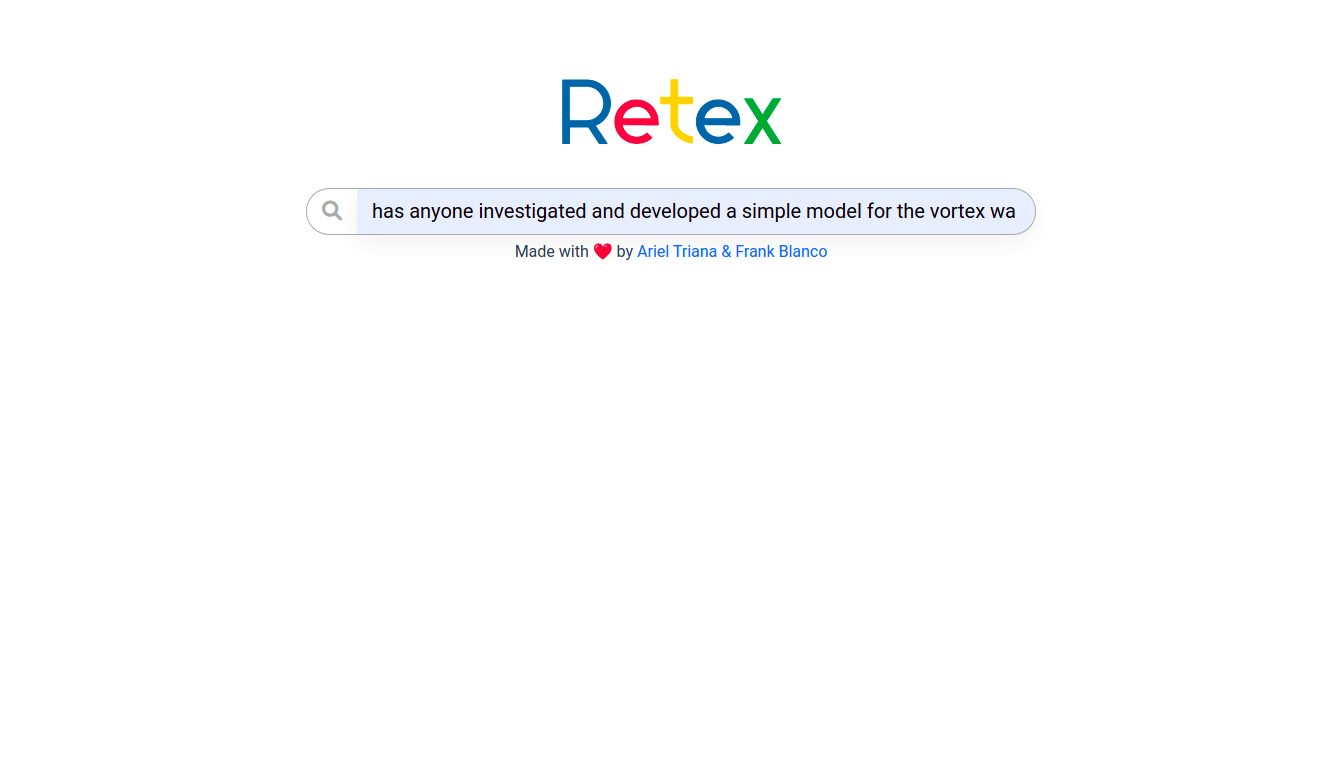
\includegraphics[width=10cm]{sections/img/home.png}
    \caption{Página de inicio de la interfaz visual con una consulta}
\end{figure}

\begin{figure}
    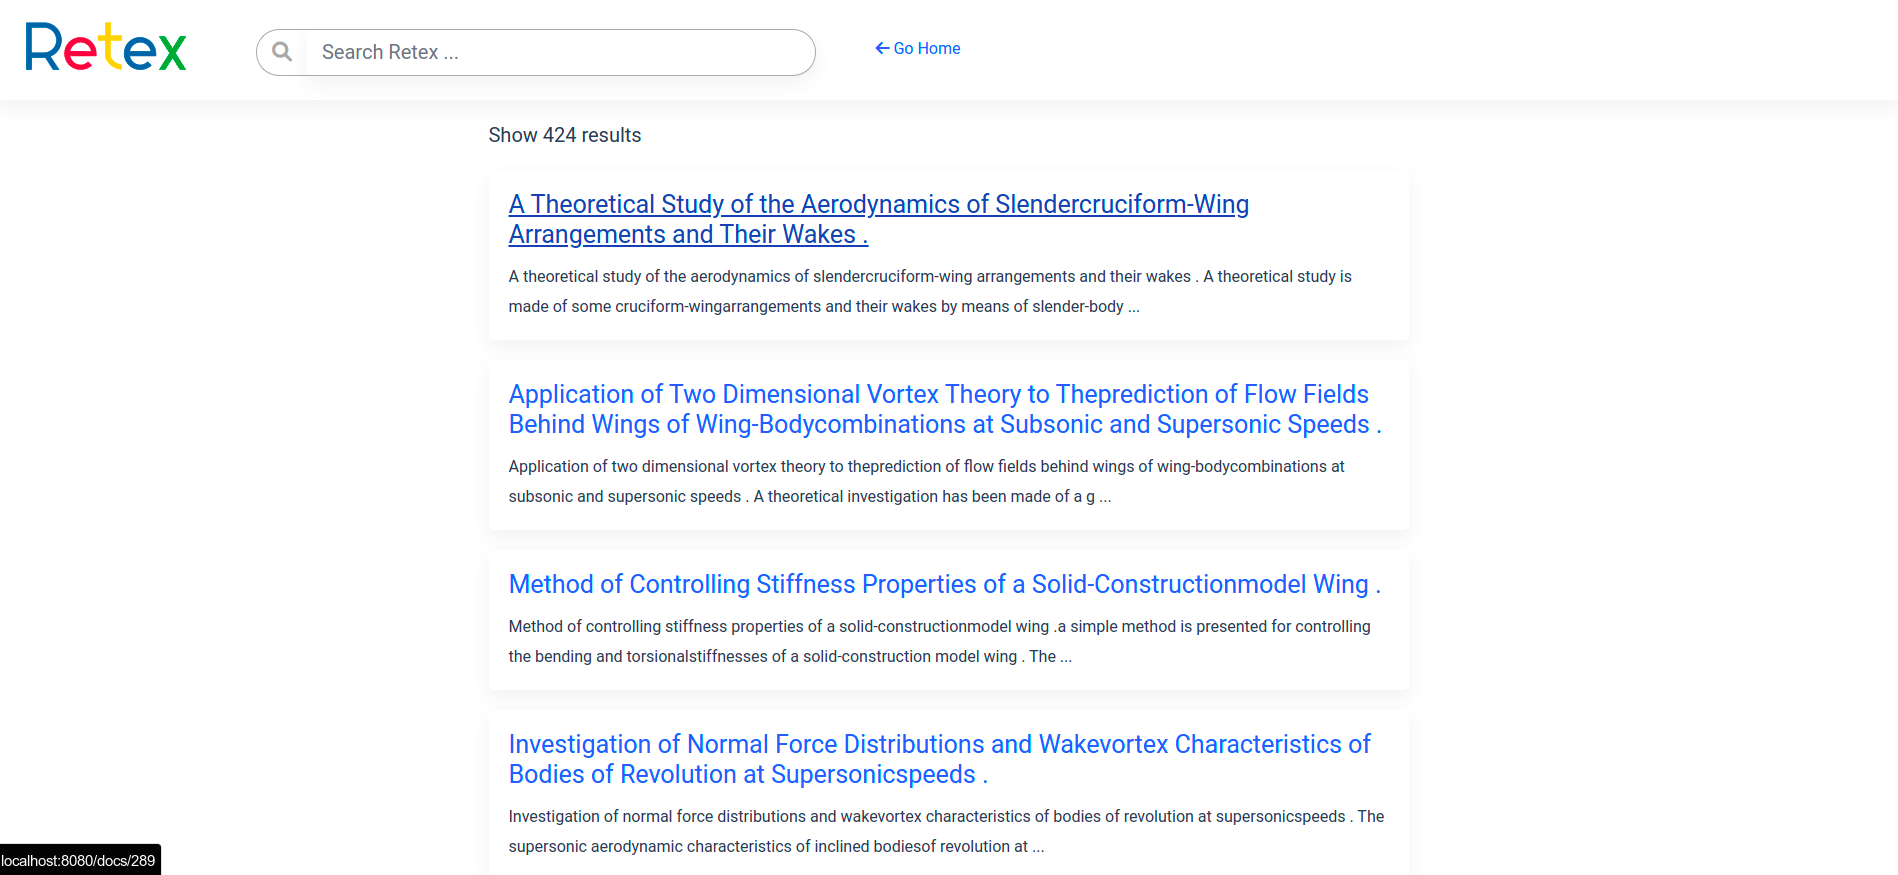
\includegraphics[width=10cm]{sections/img/result.png}
    \caption{Resultado del motor de búsqueda para la consulta realizada}
\end{figure}


    \section{Conclusiones}

Entre las ventajas del modelo implementado, podemos decir que su tiempo de respuesta es bastante rápido lo cual constituye una de las medidas subjetivas de evaluación. Además su interfaz visual es bastante intuitiva por tanto el usuario final que utiliza ReTex no tiene que realizar grandes esfuerzos para realizar una consulta al sistema. Además el modelo se basa en las métricas Tf-Idf para darle peso a los términos. Pero también presenta deficiencias el sistema. La primera es que considera a los términos indexados como independientes. Sabemos que en la realidad sí existe correlación entre  algunos. Por ejemplo si analizamos las palabras sistema y computación es probable que en un texto especializado aparezcan frecuentemente correlacionados. Esta presunción del modelo vectorial aunque pueda parecer una  limitación simplifica el proceso de recuperación y en algunos casos mejora su rendimiento. El análisis de correlación de términos requiere de enfoques más avanzados y está sujeto al contexto y la naturaleza de los documentos en términos de variedad temática, por ejemplo. Otra de las deficiencias es que el modelo del motor de búsqueda es estático por tanto, si se añaden nuevos documentos al sistema utilizando mecanismos vistos en conferencias como los Crawlers, se tendría que calcular todo el modelo nuevamente lo cual sería costoso. Además, toda consulta debe tener al menos un término en común con alguno de los documentos, si no la función $sim$ sería 0.

\section{Recomendaciones}

Entre las recomendaciones de los autores para mitigar las desventajas se encuentran las siguientes:

\begin{enumerate}
    \item[$\bullet$] El uso de word embeddings para mitigar el error de $sim = 0$ y además representar el contexto de los términos indexados.
    \item[$\bullet$] Explorar los resultados de lo siguiente: agrupar los documentos por temáticas o categorías y cuando se introduzca una consulta al motor de búsqueda se buscaría solamente entre los documentos que pertenecen a la misma temática que la consulta. Esta idea se estuvo explorando y en principio se obtuvieron resultados no muy buenos pues se escapaban documentos relevantes cuya temática principal no era la idea central de la consulta. 
    \item[$\bullet$] Añadir expansión de las consultas al sistema, para reducir el esfuerzo del usuario en la realización de las consultas.
\end{enumerate}
    % ? reference
    \begin{thebibliography}{4}
    \bibitem{mri} Blanco, F. A, Triana, A. A.: Recuperación de Información Musical: estado del arte. 2021
    \bibitem{manning} Manning, C. D., Raghavan, P., Schutze, H.: An Introduction to Information Retrieval. 2009
    \bibitem{cran} Richmond, P. A.: Review of the Cranfield project. American Documentation. 1963
    \bibitem{re} Robertson, S. E., Jones, K. S: Relevance Weighting of Search Term. 1976
    \bibitem{tf} TfidfTranform documentación \url{https://scikit-learn.org/stable/modules/generated/sklearn.feature_extraction.text.TfidfTransformer.html#sklearn.feature_extraction.text.TfidfTransformer}
    \bibitem{tfidf} TfIdfVectorizer documentación \url{https://scikit-learn.org/stable/modules/generated/sklearn.feature_extraction.text.TfidfVectorizer.html}
    \bibitem{cos} Cosine similarity documentación \url{https://scikit-learn.org/stable/modules/generated/sklearn.metrics.pairwise.cosine_similarity.html}
\end{thebibliography}
\end{document}